\tikzset{arbre3/.style = {every node/.style = {minimum size = #1, circle, draw},
                          level distance =10mm, 
                          level 1/.style={sibling distance=32mm},
                          level 2/.style={sibling distance=16mm},
                          level 3/.style={sibling distance=8mm},
                         },
         arbre3/.default=8mm
        }
\tikzset{fl/.style={ draw, fill = gray,rectangle,minimum size=3mm}}
%-------------------------------------------------------------------------------
%-------------------------------------------------------------------------------
\chapter{I -- Tracé d'arbres binaires}
%-------------------------------------------------------------------------------
%-------------------------------------------------------------------------------
\thispagestyle{empty}
%-------------------------------------------------------------------------------
%-------------------------------------------------------------------------------
{\sf 
On se propose ici de représenter des arbres binaires afin de pouvoir visualiser les opérations que l'on effectue sur ces arbres. On souhaite  dessiner les arbres de telle manière que le parcours infixe consiste à lire les nœuds (et les feuilles) de gauche à droite ; on impose aussi que les nœuds de même profondeur soient alignés horizontalement. On placera donc les nœuds sur une grille.
}

\medskip

L'objectif est de faire tracer à OCaml l'arbre (abstrait) de gauche sous la forme de droite

%-------------------------------------------------------------------------------
\begin{minipage}{8cm}
\begin{center}
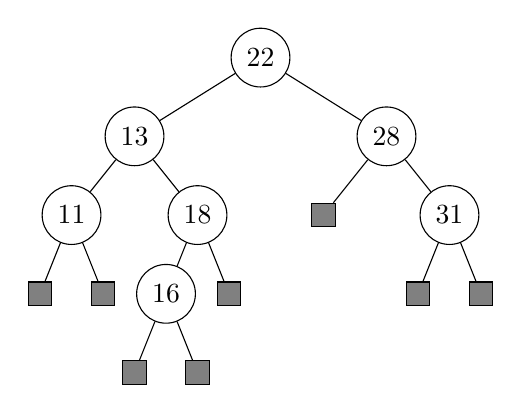
\begin{tikzpicture}[arbre3=4mm]
\node {$22$}
 child {node{$13$}
        child {node{$11$}
               child {node[fl]{}}
               child {node[fl]{}}
              }
        child {node{$18$}
               child {node{$16$}
                      child {node[fl]{}}
                      child {node[fl]{}}
                     }
               child {node[fl]{}}
              }
       }
 child {node{$28$}
        child {node[fl]{}}
        child {node{$31$}
               child {node[fl]{}}
               child {node[fl]{}}
              }
       };
\end{tikzpicture} 
\end{center}
\end{minipage}
\begin{minipage}{8cm}
\begin{center}
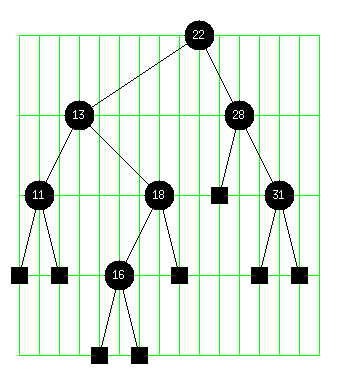
\includegraphics[scale=0.6]{arbre}
\end{center}
\end{minipage}
%-------------------------------------------------------------------------------

Nous allons travailler par renforcements successifs d'une fonction : dans chaque partie elle sera améliorée.

Le type de donnée est celle du cours pour des arbres binaires d'entiers.
%-------------------------------------------------------------------------------
\begin{ocaml}
type arbre = Vide | Noeud of arbre * int * arbre;;
\end{ocaml}
%-------------------------------------------------------------------------------
\newpage
%-------------------------------------------------------------------------------
%-------------------------------------------------------------------------------
\section{Rectangles}
%-------------------------------------------------------------------------------
%-------------------------------------------------------------------------------
%-------------------------------------------------------------------------------
Dans cette partie nous allons encadrer chaque sous-arbre dans un rectangle.

Dans un premier temps on va calculer la taille de la grille qui contient l'arbre. On a besoin
\begin{itemize}
  \item du nombre de pas verticaux, c'est la profondeur maximale des feuilles donc la hauteur augmentée de 1,
  \item du nombre de pas horizontaux, comme on dessine un nœud ou une feuille par pas, c'est le nombre total de nœuds/feuilles diminué de 1 donc le double du nombre de nœuds. (Rappel : le nombre de feuilles est le nombre de nœud plus 1.) Plus simplement si les deux fils d'un arbre non vide ont des largeurs $p$ et $q$ l'arbre aura une largeur de $p + q + 2$ car il faut placer la racine entre les deux fils.
\end{itemize}
%-------------------------------------------------------------------------------
%-------------------------------------------------------------------------------
\begin{question}{}{}
Écrire une fonction qui calcul la taille sous la forme d'un couple \type{(largeur, hauteur)}.

On ne fera qu'une lecture de l'arbre

\reponse

Comme la largeur est le nombre de nœuds/feuilles moins un, on doit ajouter 2 lors de la construction.
\begin{ocaml}
let rec taille arbre =
  match arbre with
  |Vide -> 0, 0
  |Noeud(g, r, d) -> let lg, hg = taille g 
                     and ld, hd = taille d in
                     (lg + ld + 2, max hd hg + 1);;
\end{ocaml}
\end{question}
%-------------------------------------------------------------------------------
\begin{ocaml}
taille : arbre -> int * int
\end{ocaml}
%-------------------------------------------------------------------------------
%-------------------------------------------------------------------------------
On va maintenant dessiner le cadre d'un arbre.

Pour faire des représentations graphique on a besoin de la bibliothèque graphique.
%-------------------------------------------------------------------------------
\begin{ocaml}[]
#load "graphics.cma";;
open Graphics;;
\end{ocaml}
%-------------------------------------------------------------------------------
\begin{enumerate}
  \item La première ligne charge en mémoire le fichier de la bibliothèque.
  \item La deuxième ligne permet d'utiliser les fonctions de la bibliothèque directement : on écrit \type{draw} au lieu de \type{Graphics.draw}
\end{enumerate}
%-------------------------------------------------------------------------------
Une documentation complète se trouve à

\type{https://ocaml.github.io/graphics/graphics/Graphics/index.html}

%-------------------------------------------------------------------------------
\begin{itemize}
    \item Les dessins se font dans une fenêtre que l'on doit ouvrir puis fermer.
%-------------------------------------------------------------------------------
\begin{ocaml}
open_graph " 800x900";;
...
close\_graph ();;
\end{ocaml}
%-------------------------------------------------------------------------------
Ici on a ouvert une fenêtre graphique de 800 pixels de large et 900 pixels de haut. 

L'espace blanc avant le premier chiffre est obligatoire.
%-------------------------------------------------------------------------------
\item Les coordonnées sont calculées en pixels (ce sont des entiers), 

l'origine est en bas à gauche.
%-------------------------------------------------------------------------------
\item Pour observer le dessin avant de le fermer, on pourra utiliser l'instruction
\begin{ocaml}
let _ = wait_next_event [Button_down] in close_graph();
\end{ocaml}
Elle met le programme en pause en attendant un clic de souris.
%-------------------------------------------------------------------------------
\item On définit les constantes 
%-------------------------------------------------------------------------------
\begin{ocaml}
let pas_h = 20;;
let pas_v = 80;;
let x0 = 20;;
let y0 = 800;;
\end{ocaml}
%-------------------------------------------------------------------------------
\type{pas_h} et \type{pas_v} sont les tailles, respectivement horizontale et verticale, de la grille.

$x_0$ et $y_0$ sont les coordonnées du point de départ qui correspond au point en haut et à gauche du rectangle, en effet l'arbre sera dessiné depuis sa racine.
%-------------------------------------------------------------------------------
\item On peut dessiner un rectangle avec la fonction \type{draw_rect x y larg haut} : $x$ et $y$ sont les coordonnées du point en bas à droite, \type{larg} est la largeur, \type{larg} est la hauteur.
\end{itemize}
%-------------------------------------------------------------------------------
%-------------------------------------------------------------------------------
\begin{question}{}{}
Écrire une fonction \type{rectg x1 y1 x2 y2} qui dessine un rectangle à partir des coordonnées des points supérieur gauche et inférieur droit.
\begin{ocaml}
rectg : int -> int -> int -> int -> unit
\end{ocaml}
\reponse

\begin{ocaml}
let rectg x1 y1 x2 y2 =
draw_rect x1 y2 (x2 - x1) (y1 - y2);;
\end{ocaml}
\end{question}
%-------------------------------------------------------------------------------
%-------------------------------------------------------------------------------
%-------------------------------------------------------------------------------
\begin{question}{}{}
Écrire une fonction \type{bas_droite a b arbre} qui renvoie les coordonnées du point en bas à  droite du rectangle qui délimite l'arbre et dont le point en haut à gauche est de coordonnées $a$ et $b$.
\begin{ocaml}
bas_droite : int -> int -> arbre -> int * int
\end{ocaml}

\reponse

\begin{ocaml}
let rec bas_droite a b arbre =
  match arbre with
  |Vide -> a, b
  |Noeud(g, r, d)-> 
            let xg, yg = bas_droite a (b - pas_v) g in
            let xd, yd = bas_droite (xg + 2*pas_h) 
                                    (b - pas_v) d in
  xd, min yg yd;;
\end{ocaml}
\end{question}
%-------------------------------------------------------------------------------
%-------------------------------------------------------------------------------
%-------------------------------------------------------------------------------

Voici une fonction qui dessine le rectangle délimitant un arbre.
%-------------------------------------------------------------------------------
\begin{ocaml}
let rectangle arbre =
  let x2, y2 = bas_droite x0 y0 arbre in
  open_graph " 800x900";
  rectg x0 y0 x2 y2;
  let _ = wait_next_event [Button_down] in close_graph ();;
\end{ocaml}
%-------------------------------------------------------------------------------

\begin{minipage}{0.5\textwidth}
%-------------------------------------------------------------------------------
%-------------------------------------------------------------------------------
\begin{question}{}{}
Écrire une fonction \type{rectangles arbre} qui dessine tous les rectangles délimitant les sous-arbres non réduits à une feuille.
\begin{ocaml}
rectangles : arbre -> unit
\end{ocaml}

\reponse

\begin{ocaml}
let rectangles arbre =
    let rec aux x y a =
        match a with
        |Vide -> x, y
        |Noeud(g, r, d)-> 
                let x1, y1 = aux x (y - pas_v) g in
                let x2, y2 = aux (x1 + 2*pas_h) 
                                 (y - pas_v) d in
                let yy = min y1 y2 in
                rectg x y x2 yy;
                x2, yy in
    open_graph " 800x900";
    let _ = aux x0 y0 arbre in
    let _ = wait_next_event [Button_down] in close_graph ();;
\end{ocaml}

\newpage
\end{question}
%-------------------------------------------------------------------------------
%-------------------------------------------------------------------------------
La fonction devra faire appel à une fonction récursive adaptée de \type{bas_droite}, afin de pouvoir encadrer la fonction récursive par l'ouverture et la fermeture de la fenêtre. Cette fonction récursive aura comme paramètres les coordonnées du coin supérieur gauche du rectangle qui délimite l'arbre, pour l'arbre global ces coordonnées sont $x_0$ et $y_0$.
\end{minipage}
%-------------------------------------------------------------------------------
\begin{minipage}{0.5\textwidth}
\begin{center}
\begin{tikzpicture}[scale=0.4]
  \draw (0, 0) rectangle (14, 16) ;
  \draw (0, 0) rectangle (8, 12) ;
  \draw (0, 4) rectangle (2, 8) ;
  \draw (4, 0) rectangle (6, 4) ;
  \draw (4, 0) rectangle (8, 8) ;
  \draw (10, 4) rectangle (14, 12) ;
  \draw (12, 4) rectangle (14, 8) ;
\end{tikzpicture}
\end{center}
\end{minipage}
%-------------------------------------------------------------------------------
\newpage
%-------------------------------------------------------------------------------
%-------------------------------------------------------------------------------
\section{Tracé}
%-------------------------------------------------------------------------------
%-------------------------------------------------------------------------------
\subsection{Squelette}
%-------------------------------------------------------------------------------
%-------------------------------------------------------------------------------
%-------------------------------------------------------------------------------
On souhaite maintenant tracer le squelette de l'arbre, c'est-à-dire l'ensemble des segments entre les nœuds et leurs fils (vides ou non).

\begin{minipage}{0.6\textwidth}
Pour dessiner des segments on utilise 2 fonctions de déplacement :

\begin{itemize}
  \item \type{moveto x y} déplace la position sans rien tracer jusqu'à $(x,y)$
  \item \type{lineto x y} trace un trait depuis la position actuelle jusqu'a $(x,y)$ .
\end{itemize}

%-------------------------------------------------------------------------------
%-------------------------------------------------------------------------------
\begin{question}{}{}
Écrire une fonction \type{squelette arbre} qui dessine tous les segments.

Une fonction auxiliaire pourra renvoyer aussi la position de la racine.
\begin{ocaml}
squelette : arbre -> unit
\end{ocaml}

\reponse

\begin{ocaml}
let squelette arbre =
    let rec aux x y a =
        match a with
        |Vide -> x, y, x
        |Noeud(g, r, d)-> 
                let x1, y1, xr1 = aux x (y - pas_v) g in
                let x2, y2, xr2 = aux (x1 + 2*pas_h) 
                                      (y - pas_v) d in
                moveto xr1 (y -pas_v);
                lineto (x1 + pas_h) y;
                lineto xr2 (y -pas_v);
                x2, (min y1 y2), (x1 + pas_h) in
    open_graph " 800x900";
    let _ = aux x0 y0 arbre in
    let _ = wait_next_event [Button_down] in close_graph ();;
\end{ocaml}
\end{question}
%-------------------------------------------------------------------------------
%-------------------------------------------------------------------------------
%-------------------------------------------------------------------------------
\end{minipage}
%-------------------------------------------------------------------------------
\begin{minipage}{0.4\textwidth}
\begin{center}
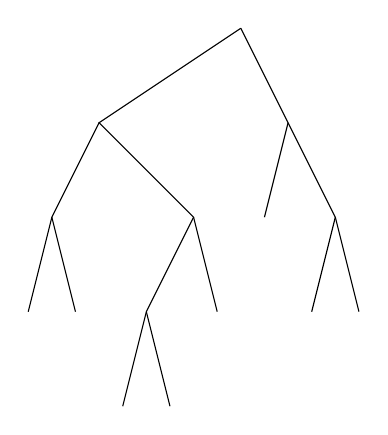
\begin{tikzpicture}[scale=0.3]
  \draw (9, 0) -- (3, -4) -- (7, -8) -- (5, -12) -- (4, -16);
  \draw (5, -12) -- (6, -16);
  \draw (7, -8) -- (8, -12);
  \draw (3, -4) -- (1, -8) -- (0, -12);
  \draw (1, -8) -- (2, -12);
  \draw (9, 0) -- (11, -4) -- (13, -8) -- (14, -12);
  \draw (11, -4) -- (10, -8);
  \draw (13, -8) -- (12, -12);
\end{tikzpicture}
\end{center}
\end{minipage}
%-------------------------------------------------------------------------------
%-------------------------------------------------------------------------------
\subsection{Nœuds}
%-------------------------------------------------------------------------------
%-------------------------------------------------------------------------------
%-------------------------------------------------------------------------------
\begin{minipage}{0.7\textwidth}
On va maintenant placer les nœuds et les feuilles. Un nœud sera représenté par un disque de rayon 15 (par exemple) et une feuille par un carré de longueur 16, ces formes seront centrées aux extrémités des segments.
\begin{ocaml}
let cote = 16
let rayon = 15;;
\end{ocaml}
%-------------------------------------------------------------------------------
\begin{question}{}{}
Écrire une une fonction de dessin de la racine d'un arbre à la position $(x, y)$.
\begin{ocaml}
dessinNoued arbre -> int -> int -> unit
\end{ocaml}
\reponse
\begin{ocaml}
let dessinNoeud arbre x y =
  match arbre with
  |Vide ->  fill_rect (x-cote/2) (y-cote/2) cote cote
  |Noeud(g, r, d) ->  fill_circle x y rayon;;
\end{ocaml}
\end{question}

\end{minipage}
%-------------------------------------------------------------------------------
\begin{minipage}{0.3\textwidth}
\begin{center}
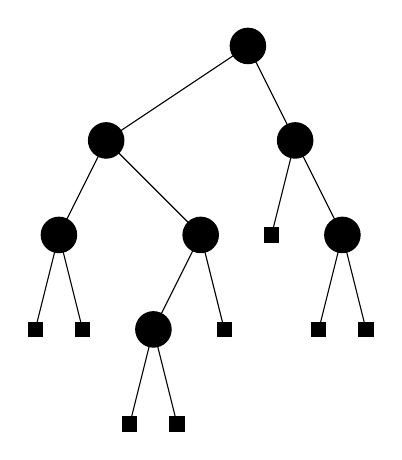
\begin{tikzpicture}[scale=0.3]
  \draw (9, 0) -- (3, -4) -- (7, -8) -- (5, -12) -- (4, -16);
  \draw (5, -12) -- (6, -16);
  \draw (7, -8) -- (8, -12);
  \draw (3, -4) -- (1, -8) -- (0, -12);
  \draw (1, -8) -- (2, -12);
  \draw (9, 0) -- (11, -4) -- (13, -8) -- (14, -12);
  \draw (11, -4) -- (10, -8);
  \draw (13, -8) -- (12, -12);
  \foreach \x/\y in {9/0, 3/-4, 11/-4, 1/-8, 7/-8, 13/-8, 5/-12} {\draw[fill] (\x, \y) circle (0.75);};
  \foreach \x/\y in {0/-12, 2/-12, 4/-16, 6/-16, 8/-12, 10/-8, 12/-12, 14/-12} 
      {\draw[fill] (\x  -0.3, \y - 0.3) rectangle (\x + 0.3, \y + 0.3);};
\end{tikzpicture}
\end{center}
\end{minipage}
%-------------------------------------------------------------------------------
%-------------------------------------------------------------------------------
\begin{question}{}{}
Écrire une fonction \type{seg_noeuds arbre} qui dessine les segments et les nœuds.

\reponse
\begin{ocaml}
let seg_noeuds arbre =
    let rec aux x y a =
        match a with
        |Vide -> dessinNoeud a x y;
                 x, y, x
        |Noeud(g, r, d)-> 
                let y0 = y - pas_v in
                let x1, y1, xr1 = aux x 0 g in
                let x2, y2, xr2 = aux (x1 + 2*pas_h) y0 d in
                let xr = x1 + pas_h in
                moveto xr1 y0;
                lineto xr y;
                lineto xr2 y0;
                dessinNoeud a xr y;
                 x2, (min y1 y2), xr in
    open_graph " 800x900";
    let _ = aux x0 y0 arbre in
    let _ = wait_next_event [Button_down] in  close_graph ();;
\end{ocaml}
\end{question}
%-------------------------------------------------------------------------------

%-------------------------------------------------------------------------------
\begin{ocaml}
seg_noeuds: arbre -> unit
\end{ocaml}
%-------------------------------------------------------------------------------
%-------------------------------------------------------------------------------
%-------------------------------------------------------------------------------
\subsection{Valeur des nœuds}
%-------------------------------------------------------------------------------
%-------------------------------------------------------------------------------
%-------------------------------------------------------------------------------

Il reste alors à écrire la valeur du nœud dans le cercle.

On utilise les fonctions 
%-------------------------------------------------------------------------------
\begin{itemize}
  \item \type{draw_string texte} qui écrit un texte avec la couleur courante depuis la position actuelle (elle correspond au point en bas à gauche).
  \item \type{string_of_int} qui convertit un entier en chaîne de caractères.
\end{itemize}
%-------------------------------------------------------------------------------

%-------------------------------------------------------------------------------
\begin{question}{}{}
Écrire une fonction \type{dessin arbre} qui dessine les segments et les nœuds ainsi que les valeurs, supposées entières, des nœuds.
\begin{ocaml}
dessin : arbre -> unit
\end{ocaml}

\reponse
On commence par modifier le dessin des nœuds pour inclure le texte.
\begin{ocaml}
let toutNoeud_r arbre x y =
    match arbre with
    |Vide ->  fill_rect (x-cote/2) (y-cote/2) cote cote
    |Noeud(g, r, d) ->  fill_circle x y rayon;
                        set_color white;
                        let ch = string_of_int r in
                        let k = String.length ch in
                        moveto (x - 3*k + 1) (y - 5);
                        draw_string ch;
                        set_color black;;
\end{ocaml}

Ensuite on dessine les nœuds des fils au lieu de celui de la racine dans la fonction, il faut alors dessiner la racine à la fin.

\begin{ocaml}
let dessin arbre =
    let rec aux x y a =
        match a with
        |Vide -> x, y, x
        |Noeud(g, r, d)-> 
                let y0 = y - pas_v in
                let x1, y1, xr1 = aux x 0 g in
                let x2, y2, xr2 = aux (x1 + 2*pas_h) y0 d in
                let xr = x1 + pas_h in
                moveto xr1 y0;
                lineto xr y;
                lineto xr2 y0;
                toutNoeud_r g xr1 y0;
                toutNoeud_r d xr2 y0;
                 x2, (min y1 y2), xr in
    open_graph " 800x900";
    let a, b, xr = aux x0 y0 arbre in toutNoeud_r arbre xr y0;
    let _ = wait_next_event [Button_down] in  close_graph ();;
\end{ocaml}
\end{question}
%-------------------------------------------------------------------------------
\newpage
%-------------------------------------------------------------------------------
%-------------------------------------------------------------------------------
\section{Décoration}
%-------------------------------------------------------------------------------
%-------------------------------------------------------------------------------
%-------------------------------------------------------------------------------
\subsection{Squelette}
%-------------------------------------------------------------------------------
%-------------------------------------------------------------------------------
\begin{minipage}{0.5\textwidth}
On peut décorer les lignes du squelette (ces fonctions agissent aussi sur les rectangles) :

\begin{itemize}
  \item \type{set\_color} sélectionne la couleur, les couleurs de base sont pré-définies :
  
  \type{black, while, red, green, blue,}
 
  \type{yellow, cyan, magenta}.
  \item \type{set\_line\_width} sélectionne la largeur du trait.
\end{itemize}
%-------------------------------------------------------------------------------
%-------------------------------------------------------------------------------
\begin{question}{}{}
Écrire une fonction \type{squelette2 arbre} qui dessine les segments.

Les segments vers des nœuds non vides seront plus épais, ceux vers une feuille seront rouge.

\begin{ocaml}
squelette : arbre -> unit
\end{ocaml}

\reponse

Il est utile d'écrire une fonction séparée pour tracer un segment selon sa destination.


\begin{ocaml}
let segment x1 y1 x2 y2 a =
    match a with
    |Vide -> moveto x1 y1;
             set_color red;
             set_line_width 1;
             lineto x2 y2
    |_ -> moveto x1 y1;
          set_color black;
          set_line_width 2;
          lineto x2 y2;;
\end{ocaml}

\begin{ocaml}
let squelette2 arbre =
    let rec aux x y a =
        match a with
        |Vide -> x, y, x
        |Noeud(g, r, d)-> 
                let y0 = y - pas_v in
                let x1, y1, xr1 = aux x y0 g in
                let x2, y2, xr2 = aux (x1 + 2*pas_h) y0 d in
                let xr = x1 + pas_h in
                segment xr y xr1 y0 g;
                segment xr y xr2 y0 d;
                dessinNoeud a xr y;
                x2, (min y1 y2), xr in
    open_graph " 800x900";
    let _ = aux x0 y0 arbre in
    let _ = wait_next_event [Button_down] in  close_graph ();;
\end{ocaml}
\end{question}
%-------------------------------------------------------------------------------
\end{minipage}
%-------------------------------------------------------------------------------
\begin{minipage}{0.5\textwidth}
\begin{center}
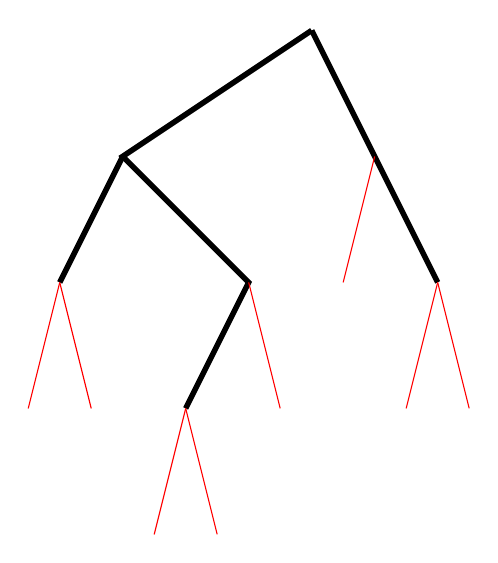
\begin{tikzpicture}[scale=0.4]
  \draw[line width = 2] (9, 0) -- (3, -4) -- (7, -8) -- (5, -12);
  \draw[line width = 2] (3, -4) -- (1, -8);
  \draw[line width = 2] (9, 0) -- (11, -4) -- (13, -8);
  \draw[color = red] (5, -12) -- (4, -16);
  \draw[color = red] (5, -12) -- (6, -16);
  \draw[color = red] (7, -8) -- (8, -12);
  \draw[color = red]  (1, -8) -- (0, -12);
  \draw[color = red]  (1, -8) -- (2, -12);
  \draw[color = red] (13, -8) -- (14, -12);
  \draw[color = red] (11, -4) -- (10, -8);
  \draw[color = red] (13, -8) -- (12, -12);
\end{tikzpicture}
\end{center}
\end{minipage}
%-------------------------------------------------------------------------------
%-------------------------------------------------------------------------------
\subsection{Noeuds}
%-------------------------------------------------------------------------------
%-------------------------------------------------------------------------------
\begin{minipage}{0.5\textwidth}
On va parfois dessiner les nœuds en couleur.
%-------------------------------------------------------------------------------
\begin{question}{}{}
Écrire une fonction \type{seg_noeudsRN arbre} qui dessine les segments et les nœuds avec les nœuds en rouge et les feuilles en noir.
\begin{ocaml}
seg_noeudsRN : arbre -> unit
\end{ocaml}
%-------------------------------------------------------------------------------

\reponse

On commence par modifier le dessin des nœuds.
\begin{ocaml}
let dessinNoeudRN arbre x y =
    match arbre with
    |Vide ->  fill_rect (x-cote/2) (y-cote/2) cote cote
    |Noeud(g, r, d) ->  set_color red;
                        fill_circle x y rayon;
                        set_color black;;
\end{ocaml}

Ensuite on dessine les nœuds des fils au lieu de celui de la racine dans la fonction, il faut alors dessiner la racine à la fin.

\begin{ocaml}
let seg_noeudsRN arbre =
    let rec aux x y a =
        match a with
        |Vide -> x, y, x
        |Noeud(g, r, d)-> 
                let y0 = y - pas_v in
                let x1, y1, xr1 = aux x 0 g in
                let x2, y2, xr2 = aux (x1 + 2*pas_h) y0 d in
                let xr = x1 + pas_h in
                moveto xr1 y0;
                lineto xr y;
                lineto xr2 y0;
                dessinNoeudRN g xr1 y0;
                dessinNoeudRN d xr2 y0;
                 x2, (min y1 y2), xr in
    open_graph " 800x900";
    let a, b, xr = aux x0 y0 arbre 
      in dessinNoeudRN arbre xr y0;
    let _ = wait_next_event [Button_down] in close_graph ();;
\end{ocaml}
\newpage
\end{question}
%-------------------------------------------------------------------------------

%-------------------------------------------------------------------------------
Si on n'y prend pas garde les segment sont dessinés au-dessus des nœuds, il faudra adapter le dessin.
%-------------------------------------------------------------------------------
\end{minipage}
%-------------------------------------------------------------------------------
\begin{minipage}{0.5\textwidth}
\begin{center}
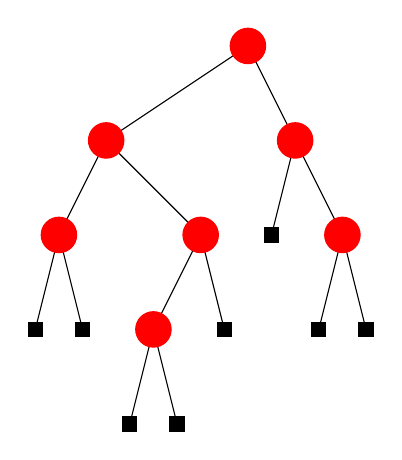
\begin{tikzpicture}[scale=0.3]
  \draw (9, 0) -- (3, -4) -- (7, -8) -- (5, -12) -- (4, -16);
  \draw (5, -12) -- (6, -16);
  \draw (7, -8) -- (8, -12);
  \draw (3, -4) -- (1, -8) -- (0, -12);
  \draw (1, -8) -- (2, -12);
  \draw (9, 0) -- (11, -4) -- (13, -8) -- (14, -12);
  \draw (11, -4) -- (10, -8);
  \draw (13, -8) -- (12, -12);
  \foreach \x/\y in {9/0, 3/-4, 11/-4, 1/-8, 7/-8, 13/-8, 5/-12} 
      {\draw[fill, color = red] (\x, \y) circle (0.75);};
  \foreach \x/\y in {0/-12, 2/-12, 4/-16, 6/-16, 8/-12, 10/-8, 12/-12, 14/-12} 
      {\draw[fill] (\x  -0.3, \y - 0.3) rectangle (\x + 0.3, \y + 0.3);};
\end{tikzpicture}
\end{center}
\end{minipage}
%-------------------------------------------------------------------------------

